\documentclass{exam}
\usepackage[utf8]{inputenc}
\usepackage{amsmath}
\usepackage{amssymb}
\usepackage{graphicx}
\usepackage{multicol}

\newcommand{\class}{MAT -- 112}
\newcommand{\term}{Spring 2018}
\newcommand{\examnum}{Review 2 Solution}
\newcommand{\examdate}{Dates: 3/14 -- 3/19}

\pagestyle{head}
\firstpageheader{}{}{}
\runningheader{\textbf{Start Time:}}{\textbf{End Time:}}{}
\runningheadrule

\begin{document}

\noindent
\begin{tabular*}{\textwidth}{l @{\extracolsep{\fill}} r @{\extracolsep{6pt}} l}
\textbf{\class} & \textbf{Name:} & \makebox[2in]{\hrulefill}\\
\textbf{\term} &&\\
\textbf{\examnum} &&\\
\textbf{\examdate} & \textbf{Pledge:}	& \makebox[2in]{\hrulefill}\\
\end{tabular*}\\
\rule[2ex]{\textwidth}{2pt}

\begin{center}
\fbox{\fbox{\parbox{5.5in}{\centering
Each question topic and the point value is recorded in the tables below. You may review these topics from any resource at your leisure. Once you decide to start a review problem, you are on the clock and you must work without any external resources, including no calculator. Each problem can be done one at a time but must be finished in a single sitting. Answer each question in the space provided; if you run out of space, then you may continue on the back of the page. It is your responsibility to plan out your time to ensure that you can finish all problems within the $4.0$ hours allotted. By writing your name and signing the pledge you are stating that your work adheres to these terms and the Davidson honor code. }}}
\end{center}

\vspace*{1em}

\begin{multicols}{2}
%% Scoring Table
\centering
\textbf{Scoring Table}\\
\addpoints
\gradetable[v][questions]

\columnbreak
%% Topics Table
\centering
\textbf{Topics Table}\\
\renewcommand{\arraystretch}{1.5}
\begin{tabular}{| c | c |}
\hline
Question & Topic\\
\hline
1 & Continuity\\
\hline
2 &The Derivative\\
\hline
3 &  Derivative Rules\\
\hline
4 & Applications \\
\hline
&\\
\hline
\end{tabular}
\end{multicols}

\vspace*{2em}
%%Time Table
\begin{center}
\textbf{Time Table}\\
\renewcommand{\arraystretch}{2.5}
\begin{tabular}{| c | c | c | c | c | c | c | c | c | }
\hline
Question & ~~~~1~~~~ & ~~~~2~~~~ & ~~~~3~~~~ & ~~~~4~~~~ \\
\hline
Time & & & &  \\
\hline
\end{tabular}
\end{center}

\newpage

\begin{questions}

\question Let $f$ be a function defined over the real numbers. 
\begin{parts}
\part[2] State the limit definition of $f$ being continuous at a real number $c$.~\\~\\
\textbf{Solution:} The function $f$ is continuous at the real number $c$ if $f(c)$ exists, $\lim_{x\rightarrow x}f(x)$ exists, and
\[
\lim_{x\rightarrow c}f(x)=f(c).
\]
\vspace{\stretch{1}}
\part[2] Use the definition in (a) to find and justify where the function below is discontinuous.

\begin{figure}[h]
\centering
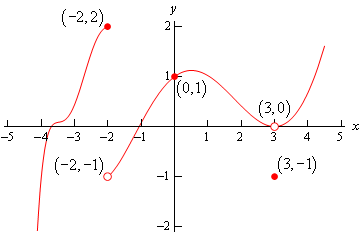
\includegraphics[scale=0.5]{review2_fig2}
\end{figure}
~\\~\\
\textbf{Solution:} The function $f$ is discontinuous at $x=-2$ since $\lim_{x\rightarrow -2}f(x)$ does not exists (the right and hand left hand limits are unequal). In addition, the function $f$ is discontinuous at $x=3$. While $\lim_{x\rightarrow 3}=0$ it is also true that $f(3)=-1$. Since these values are not equal, it follows that the function is discontinuous at $x=3$. 
\vspace{\stretch{1}}

\part[6] Suppose that $f$ is a polynomial. Then, use limit rules and the definition in (a) to show that $f$ is continuous at every real number $c$.~\\~\\
\textbf{Solution:} Let $p(x)=a_{0}+a_{1}x+\cdots+a_{m}x^{m}$ be a polynomial of degree $m$. Then for any real number $c$ we have
\begin{align*}
\lim_{x\rightarrow c}p(x)&=\lim_{x\rightarrow c}\sum_{i=0}^{m}a_{i}x^{i}\quad\text{(definition of polynomial)} \\
&=\sum_{i=0}^{m}\lim_{x\rightarrow c}a_{i}x^{i}\quad\text{(limit sum rule)} \\
&=\sum_{i=0}^{m}a_{i}\lim_{x\rightarrow c}x^{i}\quad\text{(limit constant multiple rule)} \\
&=\sum_{i=0}^{m}a_{i}c^{i}\quad\text{(limit product rule)} \\
&=p(c).
\end{align*}
\vspace{\stretch{2}}
\end{parts}

\newpage

\question Let $f$ be a function defined over the real numbers.
\begin{parts}
\part[2] State the limit definition of the derivative, if it exists, of $f$ at a real number $x$. ~\\
\textbf{Solution:} The function $f$ is differentiable at $x$ if and only if the following limit exists
\[
f^{'}(x)=\lim_{h\rightarrow 0}\frac{f(x+h)-f(x)}{h}.
\]
\vspace{\stretch{1}}
\part[4] Let $f(x)=\sqrt{x}$. Then, use the definition in (a) to find the derivative of $f$.~\\
\textbf{Solution:} Following the definition in (a) we have
\begin{align*}
f^{'}(x)&=\lim_{h\rightarrow 0}\frac{\sqrt{x+h}-\sqrt{x}}{h} \\
&=\lim_{h\rightarrow 0}\frac{\sqrt{x+h}-\sqrt{x}}{h}\left(\frac{\sqrt{x+h}+\sqrt{x}}{\sqrt{x+h}+\sqrt{x}}\right) \\
&=\lim_{h\rightarrow 0}\frac{h}{h(\sqrt{x+h}+\sqrt{x})} = \frac{1}{2\sqrt{x}}.
\end{align*}
\vspace{\stretch{2}}
\part[4] Let $f(x)=|x|$. Then, use the definition in (a) to show that $f^{'}(0)$ does not exist. ~\\
\textbf{Solution:} Following the definition in (a), in order for $f^{'}(0)$ to exist the following limit must exist
\[
\lim_{h\rightarrow 0}\frac{|0+h|-|0|}{h} = \lim_{h\rightarrow 0}\frac{|h|}{h}.
\]
But this limit does not exist, since the limit from the left is $-1$ and the limit from the right is $+1$. Therefore, $f^{'}(0)$ does not exist.
\vspace{\stretch{2}}
\end{parts}

\newpage

\question
\begin{parts}
\part[6] Find the derivative of 
\[
f(x)=(x^{2}-1)^{3}\frac{\sqrt{-2x^{2}+1}}{3x^{4}-2}.
\]
Identify at least one place where you use the sum, constant multiple, product, power, quotient, and chain rule.~\\
\textbf{Solution:} Using the product, chain, and power rule we have
\[
f^{'}(x)=3(x^{2}-1)^{2}(2x)\frac{\sqrt{-2x^{2}+1}}{3x^{4}-2}+(x^{2}-1)^{3}\frac{d}{dx}\frac{\sqrt{-2x^{2}+1}}{3x^{4}-2}
\]
Using the quotient rule, sum, and constant multiple rule we have
\[
\frac{d}{dx}\frac{\sqrt{-2x^{2}+1}}{3x^{4}-2}=\frac{-2x}{(3x^{4}-2)\sqrt{-2x^{2}+1}}-\frac{12x^{3}\sqrt{-2x^{2}+1}}{(3x^{4}-2)^{2}}
\]
Therefore, 
\[
f^{'}(x)=3(x^{2}-1)^{2}(2x)\frac{\sqrt{-2x^{2}+1}}{3x^{4}-2}+(x^{2}-1)^{3}\left(\frac{-2x}{(3x^{4}-2)\sqrt{-2x^{2}+1}}-\frac{12x^{3}\sqrt{-2x^{2}+1}}{(3x^{4}-2)^{2}}\right).
\]
\vspace{\stretch{1}}
\part[4] Find the derivative of
\[
f(x)=\log_{4}\left(\frac{e^{\sin(x)}}{3^{\cos{x}}}\right).
\]
Identify at least one place where you use the chain rule and the logarithmic, exponential, and trigonometric derivative rules. ~\\
\textbf{Solution:} Using the chain rule and logarithmic rule we have
\[
f^{'}(x)=\frac{1}{(\ln 4)\frac{e^{\sin x}}{3^{\cos x}}}\frac{d}{dx}\frac{e^{\sin x}}{3^{\cos x}}.
\]
Using the exponential and trigonometric derivative rules (along with the quotient rule) we have
\[
\frac{d}{dx}\frac{e^{\sin x}}{3^{\cos x}}=\frac{(\cos x)e^{\sin x}3^{\cos x}-e^{\sin x}(-\ln 3\sin x)3^{\cos x}}{3^{2\cos x}}.
\]
Therefore,
\[
f^{'}(x)=\frac{1}{\ln 4}(\cos x+\ln 3\sin x).
\]
\vspace{\stretch{1}}
\end{parts}

\newpage

\question An athletic field is to be built in the shape of a rectangle $x$ units long capped by semicircle regions of radius $r$ at the two ends (e.g. see Richardson Stadium). This field is to be bounded by a $400$ meter track.
\begin{parts}
\part[4] Express the area of the rectangular portion of the field as a function of $x$ alone or $r$ alone (your choice). ~\\
\textbf{Solution.} The perimeter $P$ of the field and the area $A$ of the rectangular portion can be expressed as follows
\[
P=2x+2\pi r~\text{ and }~A=2xr.
\]
Since the perimeter is equal to $400$, it follows that $2x=400-2\pi r$. Therefore, we can write the area as a function of $r$:
\[
A(r)=400r-2\pi r^{2}. 
\]
\vspace{\stretch{1}}
\part[6] What values of $x$ and $r$ give the rectangular portion the largest possible area? ~\\
\textbf{Solution.} Note that $A(r)$ is a concave down quadratic and therefore has exactly one maximum which occurs when
\[
A^{'}(r)=400-4\pi r=0,
\]
i.e. when $r=\frac{100}{\pi}$. Therefore, $x=200-\pi r=100$, and it follows that the maximum area is
\[
A =2(100)(100/\pi),
\]
i.e. approximately $6366~m^{2}$. 
\vspace{\stretch{2}}
\end{parts}
\end{questions}

\end{document}